\chapter{The ATLAS Experiment}
\label{ch:detector}
%\epigraph{\emph{If you don’t take risks, you can’t create a future.}}{Monkey D. Luffy - One Piece}
%\epigraph{\emph{The doer and the thinker, no allowance for the other, as the failing light illuminates the mercenaries creed.}}{Jethro Tull}
\epigraph{\emph{I am just a dreamer, but you are just a dream.}}{Neil Young}
\newcommand{\pileup}{
\begin{figure}[!hbt]
\begin{center}
\subbottom[Run-1 (2011-2012)]{\includegraphics[width=0.45\textwidth]{Detector/LHC/mu_2011_2012-dec}}
\subbottom[Run-2 (2015-2018)]{\includegraphics[width=0.45\textwidth]{Detector/LHC/mu_2015_2017}}
\end{center}
\setlength{\belowcaptionskip}{-20pt}
\caption{Luminosity-weighted mean number of interaction per crossing in the \ac{ATLAS} detector during stable beams for $pp$ collisions at centre-of-mass energy of 13 \tev for (a) Run-1 (2011-2012) and (b) Run-2 (2015-2018) data collection periods.}
\label{fig:pileup}
\end{figure}
}

\newcommand{\injectionChain}{
\begin{figure}[!hbt]
\centering
\includegraphics[width=1.0\textwidth]{Detector/LHC/injector_schematics}
\setlength{\belowcaptionskip}{-20pt}
\caption{Schematics of \ac{CERN} accelerator complex. The \ac{LHC} is represented by the larger gray oval line, with the smaller machines used for early-stage accleration and to provide beams for other experiments shown in different colors~\cite{Lefevre2008}.}
\label{fig:injectionchain}
\end{figure}
}
	% --------------------------------
	% -------  THE LHC
	% --------------------------------
	The \ac{LHC} is the largest collider in the world and has been providing proton-proton ($pp$) collisions at a centre-of-mass energy of \com$=13$ \tev\ between 2015 and 2018 to several experiments situated around its ring. \ac{ATLAS} is one of the four main experiments
	\footnote{Where the other three are CMS (Compact Muon Solenoid), ALICE (A Large Ion Experiment), and LHCb (Large Hadron Collider beauty).}
	 that collects and analyses the $pp$ collision data provided by the \ac{LHC}.
	The analyses presented in this thesis have been performed using the data collected by the multi-purpose \ac{ATLAS} detector during the so-called Run-2 data taking period, that lasted between 2015 and 2018.	
	In this chapter an overview of the \ac{LHC} and \ac{ATLAS} will be presented, with a detailed focus on the most relevant components  that constitute the \ac{ATLAS} detector. 
	Section~\ref{sec:lhc} will present a general overview of the \ac{LHC} functionality and performance. 
	The overall \ac{ATLAS} detector and its constituent sub-detectors will be described in Section~\ref{sec:detector}. In Section~\ref{sec:ATLAStrig} the \ac{ATLAS} trigger system and strategy for cleverly selecting data is presented. 
	A more in-depth description of the Trigger algorithms the author has been involved in will be presented in Chapter~\ref{ch:trigger}.
	\section{The Large Hadron Collider}
	\label{sec:lhc}
	Currently, the \ac{LHC}~\cite{LHCDesignReport} is the largest and most powerful particle accelerator in the world, which has delivered approximately 160 \infb\ of $pp$ collisions data with a centre-of-mass energy of 13 \tev\ during the Run-2 data collection period which spanned between 2015 and 2018.
	The \ac{LHC} was designed to help provide answers to some of the fundamental open questions in particle physics by accessing information from collisions happening at unprecedented energies and luminosities. 
	It is located at the \ac{CERN} in Geneva, at the border between Switzerland and France, and consists of a 27-kilometre ring 50-175 meters below ground, made of superconducting magnets, with two separate beam pipes containing proton (or heavy-ion) beams travelling in opposite directions. 
	
	Strong electromagnetic fields, generated by coils made of special electric cables operating in a superconductive regime, are used to guide the particle beams around the \ac{LHC} ring. A net of 1232 superconducting dipole magnets are used to bend the beams around the ring, while 392 quadrupole magnets are used to focus the beam as it is accelerated. These magnets are kept at a temperature below 1.7 K, in order to maintain their superconductive properties and create an average magnetic field of 8.3 T. 
	\ac{RF} cavities with an electromagnetic field oscillating at 400 MHz are used to accelerate the beam particles around the ring. 
	Charged particles that pass through the cavity are affected by the \ac{EM} field, which transfers energy pushing them forward along the beam line.  
	The particle beam is not continuous, but is instead sorted into "bunches", where high (low) energy protons will arrive earlier (later) and be decelerated (accelerated) so that stay close in energy~\cite{Wille:560708}.
	
	\subsection*{Runs and performance}
	So far there have been two data collection periods ("Runs") since the \ac{LHC} first went live in 2008. 
	The first operational run, referred to as Run-1, occurred between 2009 and 2013, in which the \ac{LHC} provided 5 \infb\ and 20 \infb\ of integrated luminosity at \com= 7 \tev, and 8 \tev, respectively. 
	This was followed by a two-year upgrade program during which the \ac{LHC} was not running (\ac{LS1}). 
	During the \ac{LS1} many aspects of both the \ac{LHC} and \ac{ATLAS} detector where changed or upgraded (for example the magnets for the \ac{LHC} and the trigger system for \ac{ATLAS}) in order to handle the requirement to circulate 13 \tev\ beams and collect the resulting higher energy collision data.
	On June 2015 the \ac{LHC} restarted to deliver physics data, marking it the beginning of Run-2, which lasted until 2018.
	 In this period the \ac{LHC} collided up to $10^{11}$ bunches of protons every 25 ns, resulting in over forty million collisons per second at the design luminosity\footnote{The highest luminosity the detector was design to cope with.} of $2\times10^{34}\,\mathrm{cm}^{-2}\mathrm{s}^{-1}$.
	 Luminosity is defined as~\cite{Herr:941318}:
	\begin{equation}
		\mathcal{L}=f\frac{n_bN_1N_2}{4\pi\sigma_x\sigma_y},
	\end{equation}	 
where $n_b$ is the number of bunches in an accelerator, $N_1$ and $N_2$ are the number of protons per bunch (which in the case of the \ac{LHC} is assumed to be equal) in each colliding beam, $f$ is the revolution frequency of the bunches, and $4\pi\sigma_x\sigma_y$ is the transverse area of the bunches at the interaction point, described by the Gaussian widths in the horizontal ($\sigma_x$) and vertical dimensions ($\sigma_y$) of the beam.
The instantaneous luminosity ($\mathcal{L}$) relates to the event rate ($\frac{dN}{dt}$) and the cross section ($\sigma$) of a specific process via the equation:
	\begin{equation}
	\frac{dN}{dt}\,=\,\mathcal{L}\sigma_{\mathrm{events}}.
	\end{equation}
	The number of interaction per bunch crossing is generally referred to as \textit{pile-up} ($\mu$)~\cite{pileup}, and can be expressed as 
	\begin{equation}
	\mu=\frac{\mathcal{L}\sigma_{\mathrm{inel.}}}{n_{\textrm{bunch}}f_r},
	\end{equation}
	where $\sigma_{\mathrm{inel.}}$ is the total inelastic cross-section, $n_{\textrm{bunch}}$ is the number of circulating bunches, and $f_r$ is the bunch frequency. Figure~\ref{fig:pileup} shows the mean number of interactions per bunch crossings averaged over a specific luminosity block (\mubar) found to be ranging from 13.4 up to 37.8 during the Run-2 data taking period,  which was a significant increase from the  9.7-20.7 reached in Run-1.
	\pileup
	
	\subsection*{Accelerator stages}
	To reach their maximum energy in the \ac{LHC}, protons need to be accelerated in various stages by different smaller accelerators. 
	The first stage of proton acceleration is performed by the \ac{LINAC2}, which accelerates the protons in the beam to 50 \mev; 
	the \ac{PSB} accelerates the protons to 1.4 \gev. 
	The resulting beam is then injected into the Proton Synchrotron (PS), which brings the beams to 25 \gev, and then into the \ac{SPS}, which allows the protons to reach 450 \gev.
	At this point the beams are separated into bunches with a 25 ns spacing and introduced into the \ac{LHC} where they travel in opposite directions while accelerating to the required centre-of-mass energy of 13 \tev.
	A sketch of the machinery used for the injection and acceleration of the proton beam can be seen in Figure~\ref{fig:injectionchain}. 
	The \ac{LHC} also operates heavy ion runs, which begin the acceleration process in the \ac{LINAC3} and the \ac{LEIR}, before following the same acceleration chain as the protons.
	\injectionChain
	
	The yellow points visible along the gray oval used to represent the \ac{LHC} in the schematics shown in Figure~\ref{fig:injectionchain} represent the four large detectors situated at the collision points: the \ac{LHCb}~\cite{LHCb2008} that focuses on flavour physics; \ac{ALICE}~\cite{ALICEJINST}, which is specialised in heavy ion physics; and the multi-purpose \ac{CMS}~\cite{CMSJINST}, and \ac{ATLAS} detectors. There are many other smaller experiments situated at \ac{CERN} both in the cavers about the collision points and around the site, but these are beyond the scope of the thesis and will not be discussed further. 
	
	\section{The ATLAS detector}
	\label{sec:detector}
	The \ac{ATLAS} detector was designed to be a multi-purpose detector able to collect the data with the highest luminosity available by the \ac{LHC}. The \ac{ATLAS} detector has a forward-backward cylindrical geometry with respect to the interaction point, totalling in about 45 m in length and 25 m in diameter.  It was designed to reconstruct and measure physics objects, such as electrons, muons, photons, and hadronic jets, that are essential for the core physics programmes at the \ac{ATLAS} experiment.
	%, like \ac{BSM} searches and the Higgs boson discovery.
	Various sub-systems (sub-detectors) are used to observe all possible decay products in a nearly $4\pi$ steradians of solid angle. 
	
	\begin{figure}[!hbt]
\centering
\includegraphics[width=1.0\textwidth]{Detector/ATLAS/cut-away-det-orig}
\setlength{\belowcaptionskip}{-20pt}
\caption{Schematics of cut-away \ac{ATLAS} detector with labelled sub-systems. The dimensions of the detector are 25 m in height and 45 m for an overall weight of approximately 7000 tonnes~\cite{Lefevre2008}.}
\label{fig:ATLAS}
\end{figure}
	A schematic of the \ac{ATLAS} detector and its components is shown in Figure~\ref{fig:ATLAS}. 
	The sub-detector system closest to the interaction point is the \ac{ID}, which is a core component of the tracking system, and consists of the \ac{Pixel}, \ac{SCT}, and \ac{TRT}. 
	A 2 T magnetic field, generated by a thin superconducting solenoid which envelops the \ac{ID}, bends the trajectories of the charged particles originating from the interaction process, and thus allows for the measurement of their transverse momentum.
	The next layers of the detector are composed of the Electromagnetic and Hadronic Calorimeters, which are used to perform precise energy measurements of photons and electrons in the former, and hadronic jets in the latter. The outermost layer of the detector is composed by the \ac{MS}, which is located in a 4 T magnetic field generated by the barrel and end-cap toroids, and is tasked with the detection of tracks originating from penetrating muons. The magnets and sub-detectors that compose the \ac{ATLAS} detectors will be discussed in more detail in the following sections.  
	\subsection*{The ATLAS coordinate system}
	\label{subsec:coord}
	A coordinate system with its origin at the interaction point of the detector is used for the spatial definition of the sub-detectors and kinematic measurements of physics processes.
	The $z$-axis runs along the beam line, with the $x-y$ plane thus being perpendicular to the beam, and the $x$ and $y$ axes pointing from the origin towards: the centre of the \ac{LHC} ring, and the surface of the earth, respectively.
	
	Spherical coordinates are used, with $\phi$ being the azimuthal angle around the beam axis, and $\theta$ being the polar angle measured from the positive $z$-axis. 
	Other coordinates known as rapidity $y$ and pseudorapidity $\eta$ are used instead of $\theta$, which is susceptible to a boost in the beam direction. The angle $\phi$, on the other hand, is invariant under a boost in the beam direction. 
	Rapidity is generally used for massive objects, such as jets, and is defined as:
	\begin{equation}
	y=\frac{1}{2}\cdot\mathrm{ln}\left[\frac{E+p_z}{E-p_z}\right],
	\end{equation}
	where $E$ is the energy of the particle and $p_z$ is the $z$-component of the momentum.
	For light relativistic particles, for which masses can be neglected, the 
	rapidity can be reduced to the quantity:
	\begin{equation}
	\eta=-\mathrm{ln}\left[\mathrm{tan}\left(\frac{\theta}{2}\right)\right],
	\end{equation}
	called "pseudorapidity".
	In the $(\eta,\phi)$ space the angular distance between two objects can be defined as:
	\begin{equation}
	\Delta R = \sqrt{\Delta\eta^2+\Delta\phi^2},
	\end{equation}
	where $\Delta\eta$ and $\Delta\phi$ are the difference in pseudorapidity and azimuthal angle between the objects.
	Other widely used kinematic variables include the transverse momentum ($p_T$) and transverse missing energy \met.
	The transverse momentum describes the momentum of a particle in the transverse plane to beam line. It is thus measured in the $x-y$ plane and is defined as:
	\begin{equation}
	p_T = \sqrt{p_x^2+p_y^2},
	\end{equation}
	where $p_x$ and $p_y$ are the $x$ and $y$ components of the momentum.
	The \met, on the other hand, is used to describe the transverse momentum of all the "invisible" particles (\ie\ particles not detected by the \ac{ATLAS}) detector), since we know that the initial transverse momentum of the system was 0 and thus, due to conservation of momentum, the final transverse momentum must also be 0.
	Therefore a measured non-zero total "visible" momentum $\vec{p}^{\mathrm{vis}}_T$ indicates that there must be an equivalent amount of missing transverse momenta $\vec{p}^{\mathrm{miss}}_T$ with magnitude \met, defined as:
	\begin{equation}
	E_T^{\textrm{miss}}=|\vec{p}^{\mathrm{vis}}_T|=|\vec{p}^{\mathrm{miss}}_T|=|\sum_{i}\vec{p}^{\mathrm{vis,i}}_T|.
	\end{equation}

	\subsection{Magnet System}
	\label{subsec:magnet}
		\begin{figure}[!hbt]
		\begin{center}
	%	\subbottom[Geometry of magnet system ]{\includegraphics[width=.45\textwidth]{Detector/ATLAS/magnetSyst}}
		%\subbottom[]{
		\includegraphics[width=0.65\textwidth]{Detector/ATLAS/magnetSyst-desc-col}
		%}
		\end{center}
		%\setlength{\belowcaptionskip}{-20pt}
		\caption{Schematics of the \ac{ATLAS} magnet system used in the \ac{ATLAS} detector (taken from ~\cite{Zn})}
		\label{fig:magnets}
		\end{figure}
	The \ac{ATLAS} magnet system is composed of three separate sets of magnet, used to generate the magnetic field needed to bend the trajectory of charged particles in order to measure their momenta, the details of which will be described in more detail below. 
	Figure~\ref{fig:magnets} show the geometry of the system, which measures 26 m in length and 22 m in height, and is composed by the central solenoid located around the \ac{ID}, the barrel toroid which spans the length of the detector, and the end-cap toroids which are located at each end of the detector. 
	More details on each set of magnets is given below. 
	The magnets are made of \ac{NbTi}, a material which allows the magnets to operate in the superconductive conditions required to generate strong magnetic fields. 
	\begin{description}
	\item[The Central Solenoid:] it is located between the \ac{ID} and the \ac{ECAL}. It has an inner and outer radius of 2.46 m and 2.56 m, with an axial length of 5.8 m. It is designed to generate a 2 T axial magnetic field, used to bend charged particle trajectories as they travel trough the \ac{ID}, thus providing the \ac{ATLAS} experiment with accurate measurements of the momentum up to 100 \gev ~\cite{YAMAMOTO200853}.
	\item[Barrel and End-cap toroids:] these are the other two sets of toroid magnets used in the \ac{ATLAS} detector for the measurement of muon particles. On the outer edge of the detector, measuring 25.3 m in length and with an outer and inner diameter of 9.4 m and 20.1 m, respectively, is the barrel toroid. It is comprised of eight coils that provide 0.5 T toroidal magnetic field each acting perpendicular to the beam pipe, for a total field of 4 T, to the muon spectrometer. The end-cap toroid also provides a 4 T magnetic field, but are located at the ends of the detector, as shown in Figure~\ref{fig:magnets} in order to be able to measure the highly energetic muons travelling close to the beam pipe. The end-cap toroids are 5 m long and 10.7 m in diameter~\cite{ATLASJINST}. 
	\end{description}
	\subsection{Inner Detector}
	\label{subsec:id}
	\begin{figure}[!hbt]
		\begin{center}
		\subbottom[Overview of the \ac{ATLAS} \ac{ID} with labels and dimensions.]
		{\includegraphics[width=.45\textwidth]{Detector/ATLAS/ID/ID-overview}}
		\subbottom[Schematics of \ac{ATLAS} \ac{ID} and its sub-detectors]
		{\includegraphics[width=0.45\textwidth]{Detector/ATLAS/ID/ID}\label{fig:ID_b}}
		\end{center}
		%\setlength{\belowcaptionskip}{-20pt}
		\caption{The \ac{ATLAS} inner detector (taken from ~\cite{ATLASPhotos})}
		\label{fig:ID}
		\end{figure}
	The \ac{ID} is the sub-detector component of the \ac{ATLAS} detector closest to the interaction region. 
	It is designed to accurately reconstruct charged particle tracks used in the selection of physics objects.
	Different elements are used in the \ac{ID}, as shown by Figure~\ref{fig:ID}, to ensure that all particles within a range of $|\eta|<2.5$ and \pt\ $>0.5$ \gev\ can be measured. 
	Primary and Secondary vertices are accurately measured by the Pixel layer, composed of the \ac{Pixel} and \ac{IBL}, whose outgoing tracks are then detected by the \ac{SCT} and finally identified by the \ac{TRT}. 
	A more detail description of each section of the \ac{ID} is given below.
	\begin{description}
	\item[\ac{Pixel}:] 
	The \ac{Pixel}~\cite{Pixelbib} detector is composed of three layers of silicon pixels formed into 1,456 and 288  identical sensorchip-hybrid modules for the barrel and end-caps, respectively. 
	Each module contains 46,080 readout channels, or pixels, each with a surface area of $50\times400\,\mu\mathrm{m}^2$, for a total of approximately 80 million pixels in the whole system (barrel and end-cap)~\cite{ATLASPix}. The whole of the silicon pixel detector measures 48.4 cm in diameter and 6.2 m in length, covering $|\eta|<2.5$ in pseudorapidity with three concentric layers placed at 50.5 mm, 88.5 mm, and 122.5 mm along the barrel. Three additional layers are located at the end-caps of both ends of the \ac{ID}, for a total of 6 layers. This is done so that when a charge particle traverses the layers the three space-points can be determined and thus the track and vertices can be reconstructed. 
	\item[\ac{IBL}:] 
		The \ac{IBL}~\cite{IBLTDR} was added during the \ac{LS1} period to improve the vertex finding by a factor of ~1.4 and impact parameter reconstruction by a factor of 2 with respect to Run-1 (see Chapter~\ref{ch:trigger} for a more detail description of the performance of vertex tracking in Run 2). It is part of the Pixel section of the \ac{ID} and is comprised of 6 million channels, with each pixel measuring $50\times250\,\mu$m. 
	\item[\ac{SCT}:] 
		The \ac{SCT}~\cite{AHMAD200798} consists of four concentric barrel layers of silicon micro-strip detectors with 2,112 modules, while the end-caps have nine layers with a total of 1,976 modules, each.
		It was designed for precision measurements of positions using four points (corresponding to eight silicon layers) obtained as track hits as a particle crosses the layers, and is used for precise momentum reconstruction for pseudorapidities $|\eta|<2.5$.
		The \ac{SCT} layers are located at 299 mm, 371 mm, 443 mm, and 514 mm from the interaction point, as shown by Figure~\ref{fig:ID_b}, with each module having an intrinsic resolution of 17 $\mu$m and 580 $\mu$m in the $R-\phi$ and $z$ directions, respectively. 
		A reduced granularity can be used whist maintaining the same level of performance, compared to the pixel detector, because it is located further away from the interaction region and thus has to cope with reduced particle density.		
	\item[\ac{TRT}:]
	The \ac{TRT}~\cite{TRT2012} consists of three barrel rings, with 32 modules each, and 18 end-caps units with 224 layers. A total of 370,000 cylindrical drift tubes (straws) of 4 mm diameter and 1.44 m in length are filled with a mixture of $70\%\,\mathrm{Xe}\,+\,27\%\,\mathrm{CO}_2\,+\,3\%\,\mathrm{O}_2$. These are positioned parallel to the beam pipe in the barrel and radial in the end caps. 
	The combination of gases have been chosen and tested to have good X-ray absorption, and increase the electron drift velocity and photon quenching.
	An aluminium coat around the straws is used as the cathode, with a 30 $\mu$m gold-plated tungsten wire through the centre of the straw tube as the anode. As a charged particle travels trough the \ac{TRT}, the gas is the straw tubes is ionised causing the electrons to drift to the anode, which records this as a hit.
	The \ac{TRT} can also perform particle identification through the detection of transition radiation photons, which are emitted when highly relativistic charged particles cross boundary between mediums with different dielectric constants. In the \ac{TRT} this is done by polypropylene fibres (foils), which are interwoven the barrel (end-cap) straws, that enable the production of transition radiation in the form of X-rays. The amount of radiation produced can be used to distinguish between, \eg\ electrons and charged pions, as the amount of radiation would depend on how relativistic the charged particle is. 
	\end{description}
	\subsection{Calorimeters}
	\label{subsec:calo}
		\begin{figure}[!hbt]
		\centering
		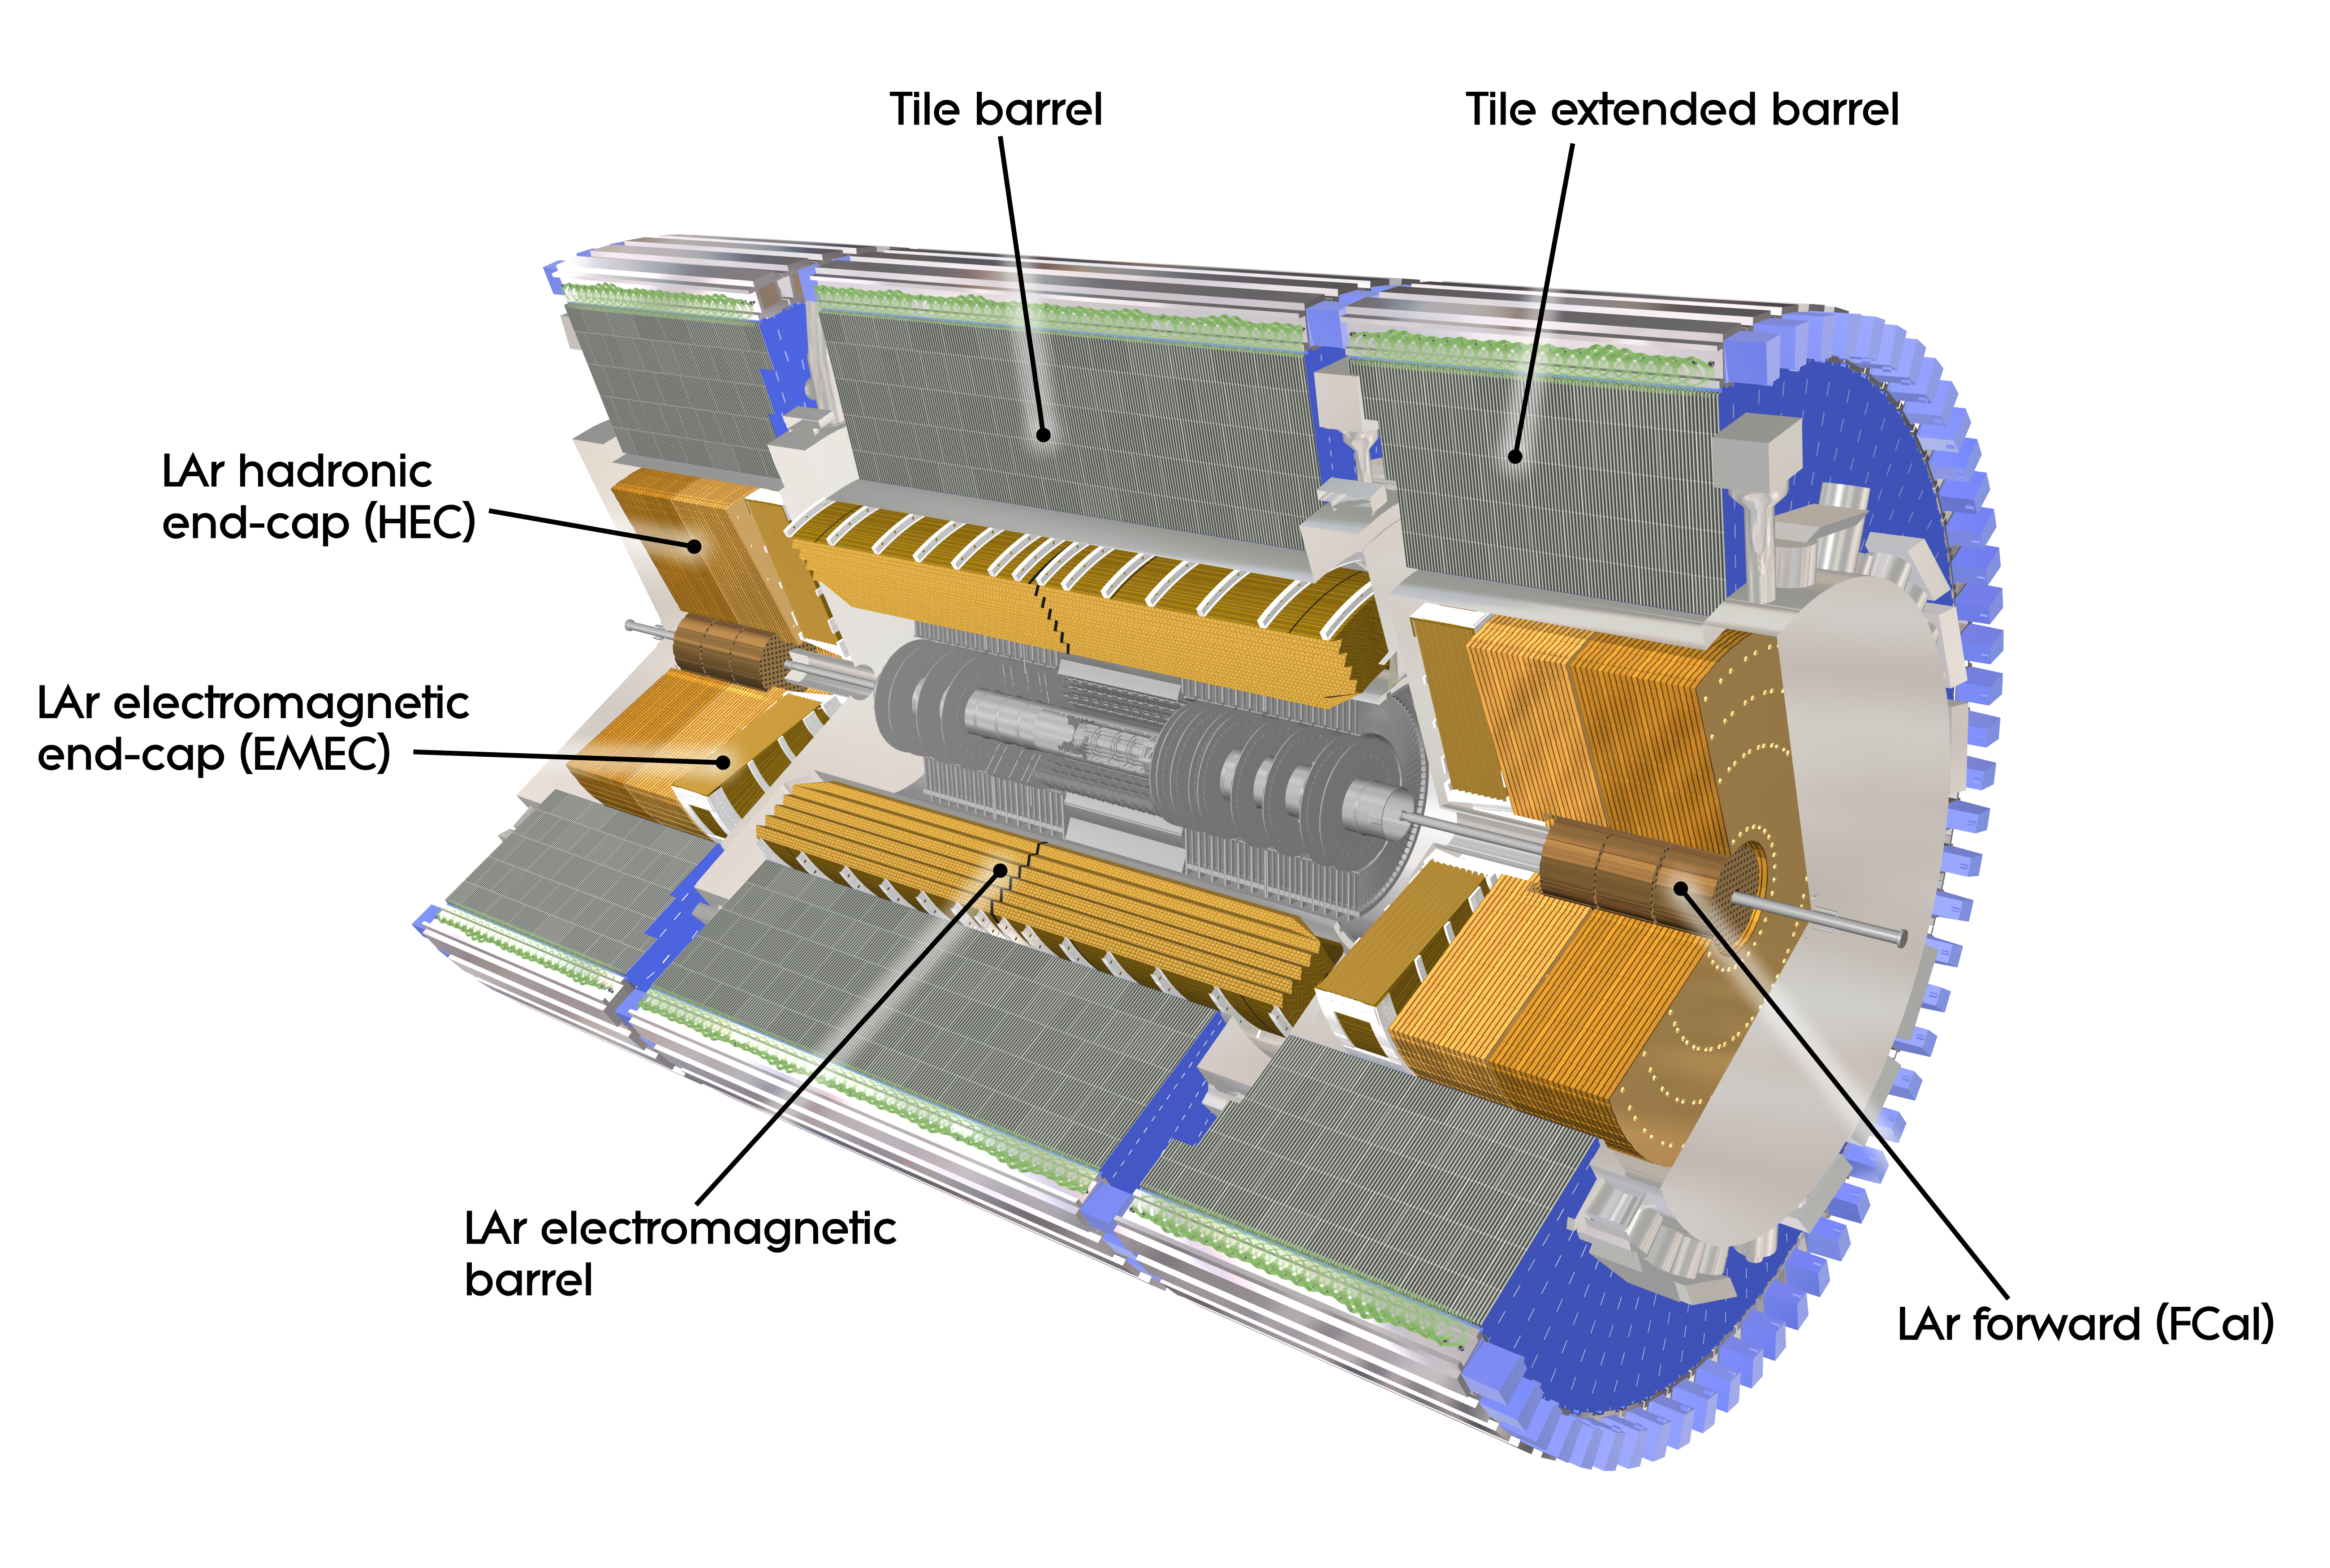
\includegraphics[width=1.0\textwidth]{Detector/ATLAS/CALO/Calo-overview_orig}
		%\setlength{\belowcaptionskip}{-20pt}
		\caption{Labelled schematics of the \ac{ATLAS} \ac{ECAL} and \ac{HCAL} system~\cite{ATLASJINST}.}
		\label{fig:calorimeters}
		\end{figure}
	The \ac{ATLAS} calorimeters are designed measure the energy of electromagnetic (\ac{ECAL}) and hadronic (\ac{HCAL}) interacting particles. 
	%The system is comprised of two main sub-detectors, the \ac{ECAL}~\cite{ATLASLAR} and \ac{HCAL}~\cite{CERN-LHCC-2017-019}, as seen by the schematics shown in Figure~\ref{fig:calorimeters}.
	The energy of electromagnetically interacting particles, such as  electrons, positrons, or photons, is measured in the \ac{ECAL}~\cite{ATLASLAR}, which is comprised of one barrel and two end-cap sensors located around the central solenoid.
	%Electromagnetically-interacting particles, such as electrons, positrons, or photons, are intercepted by the first calorimeter, comprised of one barrel and two end-cap sensors located around the central solenoid, the \ac{ECAL}. 
	The \ac{HCAL}~\cite{CERN-LHCC-2017-019} is also comprised of one barrel and two end-cap sectors and it is located around the \ac{ECAL}, so that particles travelling through the detector will have to go first go through the \ac{ECAL} and then the \ac{HCAL}. 
	It is tasked with the detection and measurement of the energy deposited by hadronic showers. 
	This is done by using tile sensors in the barrel made of scintillating plastic, while \ac{LAr} is used in the end-caps.
	Figure~\ref{fig:calorimeters} shows a detailed schematics of the calorimeter system used by the \ac{ATLAS} detector.
	More detail of the \ac{ECAL} and \ac{HCAL} geometry, functionality, and materials is given in the following paragraphs. 
	
	\begin{description}
	\item[\ac{ECAL}]
	The \ac{ECAL} utilises \ac{LAr} to measure electromagnetic showers that occur when a high-energy electron or photon travel through the fluid. 
	Photons that are above a few \mev\ will interact primarily via pair production, in which a highly energetic photon will interact with a nucleus to create a electron-positron pair. High-energy electrons and positrons, on the other hand, will produce photons via \brem. 
	These two processes will continue in the \ac{ECAL} until the energy of the emitted photons falls below the pair production threshold. At that point the energy loss of the electron will start to dominate.
	The \ac{ECAL} uses an "accordion"-geometry, shown in Figure~\ref{fig:ECAL}, comprised of multiple layers of \ac{LAr} sampler and \ac{Pb} absorber, to achieve a full $\phi$ coverage with no non-interactive regions (referred to as "cracks"), and fast extraction of signals from both front or read end of the electrodes. 
	The barrel and end-cap sectors provide a pseudorapidity coverage of up to $|\eta|<1.475$ and $1.375<|\eta|<3.20$, with the junction between the barrel and end-cap components being defined as a crack region from which any signal should be discarded. 
	An additional thin \ac{LAr} layer with no absorber is placed in front of the calorimeter in the $|\eta|<1.8$ region. 
	This layer is designed to correct for the energy lost, as particles enter the calorimeter, by taking a measurement just before the majority of the electromagnetic shower is developed. 
	\begin{figure}[!hbt]
		\centering
		\includegraphics[width=0.45\textwidth]{Detector/ATLAS/CALO/ECAL}
		%\setlength{\belowcaptionskip}{-20pt}
		\caption{Schematics of the \ac{ECAL} accordion-geometry.}
		\label{fig:ECAL}
		\end{figure}
		
	\item[\ac{HCAL}: ]
	Steel and scintillating tiles coupled with optical fibres are read out by photo-multipliers in the \ac{HCAL}.
	A central barrel, 5.64 m long covering $|\eta|<1.0$, and two extended barrels, 2.91 m long covering a region $0.8<|\eta|<1..7$ make up the \ac{HCAL}. 
	Each cylinder is composed of 64 modules, each of which is made of three layers. 
	The forward region, closest to the beam, is covered by a \ac{LAr} \ac{FCal}.
	The smallest section of the calorimeter module is a cell with a $\Delta\phi\times\Delta\eta=0.1\times0.1$ granularity for the two innermost layers and  $\Delta\phi\times\Delta\eta=0.2\times0.1$ for the outermost one.
	\end{description}
	\subsection{Muon spectrometer}
	\label{subsec:muon_spec}
	\begin{figure}[!hbt]
		\centering
		\includegraphics[width=0.9\textwidth]{Detector/ATLAS/CALO/MS}
		%\setlength{\belowcaptionskip}{-20pt}
		\caption{Computer generated schematics of the \ac{ATLAS} \ac{MS} system (taken from ~\cite{ATLASJINST}) .}
		\label{fig:muon_spectrometer}
	\end{figure}
	Muon particles are minimal interacting and are thus able to travel through the entire \ac{ATLAS} detector. 
	The \ac{MS}~\cite{MSTDR} is thus designed to accurately measure the momenta of these particles. 
	It is located within the 4 T magnetic filed generated by the long barrel toroid, described in Section~\ref{subsec:magnet}, and is comprised of three concentric chambers in the barrel region with an outer radius of 10 m, and three layers of chamber planes perpendicular to the beam pipe in the end-caps at a maximum distance of 21.5 m (as shown in Figure~\ref{fig:muon_spectrometer}). 
	High precision momentum measurements are possible by performing high precision tracking on the deflected trajectories of the charged muons as they travel through the different layers of the \ac{MS}.
	The large barrel toroid covers a region of $|\eta|<1.4$, while two end-cap toroids deflect tracks between $1.6<|\eta|<2.7$. 
	A combination of both magnets is used for the "transition" region $1.4<|\eta|<1.6$.
	Two types of chambers are used in the barrel: the \acp{MDT} and \acp{RPC}. The \acp{MDT} are also present in the end-cap layers, along with \acp{CSC} and \acp{TGC}. A more detailed description of each of the chamber systems used in the \ac{MS} is given in the following paragraphs. 
	\begin{description}
	\item[\acp{MDT}] are 29.97 mm diameter drift tubes, filled with pressurised $93\%\,\mathrm{Ar}+7\%\,\mathrm{CO}_2$ gas, employed in most of the pseudo-rapidity range to provide measurements of track coordinates in the bending direction. Electrons resulting from the ionization of the gas from a penetrating muon are collected by a tungsten-rhenium wire, measuring 50 \mum\ in diameter, located at the centre of the tube.
	Three to eight layers of drift tubes are used in both barrel and end-caps to allow a total of twenty measurements for each track. \acp{MDT} can achieve an average resolution of 80 \mum\ per tube, or about 35 \mum\ per chamber.
	\item[\acp{CSC}] are used in the innermost tracking layer for the higher particle flux and muon-track density forward direction ($2<|\eta|<2.7$), due to their higher rate capability and time resolution compared to \acp{MDT}.
	\ac{CSC} consist of two disks with eight chambers each, where each chamber contains four multi-wire proportional chambers with four cathode plates. The chambers are filled with  $80\%\mathrm{Ar}+20\%\mathrm{CO}_2$ gas, with the cathode strips aligned both parallel and perpendicular to the anode wires, to provide precision and transverse coordinates. 
	The achieved resolutions of the \ac{CSC} is 40 \mum\ in the bending plane and 5 mm in the transverse plane. 
	\item[\acp{TGC}] are very similar to \ac{CSC} and compliment the precision tracking system provided by the \ac{MDT} and \ac{CSC} by delivering track information within a few tens of nanoseconds after the passage of the particle. 
	Like \ac{CSC}, they are multiwire proportional chambers filled with $55\%\mathrm{CO_2+}$45\%n-pentane gas, with the cathode plates 2.8 mm and the anode wires 1.8 mm apart. 
	This configuration, along with high electric field, results in very good time resolutions.
	\acp{TGC} are essential for providing muon triggering and secondary complementary coordinates, orthogonal to the precision measurements, in the end-caps for the $1.05<|\eta|<2.7$ region. 
	Nine space-points are recorded for every track using a \ac{TGC}.
	\item[\acp{RPC}] are also used, like \acp{TGC}, to provide muon triggering and secondary coordinate in the barrel for $|\eta|<1.05$.
	They are parallel electrode-plate detectors, made of plastic laminate 2 mm distance apart, filled with $\mathrm{94.7\% C_2H_2F_4+5\% Iso-C_4H_{10}+0.3\% SF_6}$ gas. A maximum of six space-points are recoded for every track.
	\end{description}
	\section{The ATLAS Trigger and Data Acquisition}	
	\label{sec:ATLAStrig}
	The \ac{LHC} provides the \ac{ATLAS} experiment with $\sim$40 MHz of $pp$ collisions. 
	A sophisticated \ac{TDAQ}~\cite{TDAQRun1,TDAQRun2} system is used to reduce this rate of data down to manageable levels ($\sim$1 kHz) by storing only events that contain potentially "interesting" physics. 
	A two level trigger system has been used during Run 2, consisting of a hardware-based trigger, named \ac{L1}, and a software-based trigger, called \ac{HLT}. 
	Low granularity information from the calorimeter and muon spectrometer systems is processed by the \ac{L1} to identify so-called \acp{RoI} before making a decision. Event data from other sub-detectors and systems is stored in memory until the \ac{L1} decision is taken.
	Upon passing the rapid \ac{L1} selection, the event data is passed to the \ac{HLT} system.
	The \ac{HLT} is made of software running on computer cluster (\ac{HLT} farm), which use information not available to the \ac{L1}, such as finer-granularity calorimeter inputs and precious measurements from the \ac{MS}, to further analyse the event-data and decide whether to keep or discard the event. 
	The flow of data though the \ac{L1} and \ac{HLT} system is managed by the data acquisition system, which eventually passes all accepted events into data streams for offline physics, monitoring, and detector  analyses. 
	Objects that do not meet the \ac{L1} or \ac{HLT} requirements are discarded. 
	The \ac{ATLAS} trigger system is discussed in detail in Chapter~\ref{ch:trigger}.
	
	